\documentclass{beamer}
\usetheme{Boadilla}
%==================================================
%Mypackages
\usepackage{epsf, amsmath, amssymb, epsfig, amsthm}
\usepackage{subfigure} % For subfigures
\usepackage{setspace} 
\usepackage{fancyhdr} 
\usepackage{eurosym}  %To write a Euro symbol
\usepackage[euler]{textgreek}
\usepackage[english,main=russian,spanish]{babel}
\usepackage[utf8]{inputenc}
\usepackage{graphicx}
\usepackage{float}
\usepackage{bbm}
\usepackage{cite}
\usepackage{movie15}
\usepackage{listings}
\lstset{
  basicstyle=\ttfamily,
  columns=fullflexible,
  frame=single,
  breaklines=true,
}
\hypersetup{colorlinks,urlcolor=blue}

%==================================================
%My commands: Define your commands here:

\begin{document}
\title{Planes, Trains, and Afflictions}
\subtitle{Agent-based modeling for the spread of disease through transportation networks}
\author{NS Group 3}
\institute[ВШЭ]
{
  \inst{}%
  Faculty of Computer Science\\
  Higher School of Economics (ВШЭ)\\
  Moscow
}
\date{27 JUN 2020}
\begin{frame}
\titlepage
\end{frame}
\begin{frame}
\frametitle{Table of Contents}
\begin{itemize}
    \item Motivation
    \item Prior Research
    \item ABM Framework
    \item Examples
    \item Deep Dive: New York City (NYC) Subway
    \item Discussion
    \item Conclusion
    \item Credits
\end{itemize}
\end{frame}
\begin{frame}
\frametitle{Motivation}
Why were certain areas of NYC more affected by COVID-19?\\
How were the subways involved?\\
\textbf{image here of NYC afflictions}\\
credit: NYC DoH
\textbf{image here of line analysis}\\
credit: Jeffrey whoever mabob
\textit{Speaker's note:\\
- What is a transportation network? What is a subway?
- How infections spread on transportation networks\\
- Learn
}
\end{frame}
\begin{frame}
\frametitle{Prior Research (London Underground)}
Data: Oyster (Card), CASA (Timetable), PHE Data (Demographics)\\
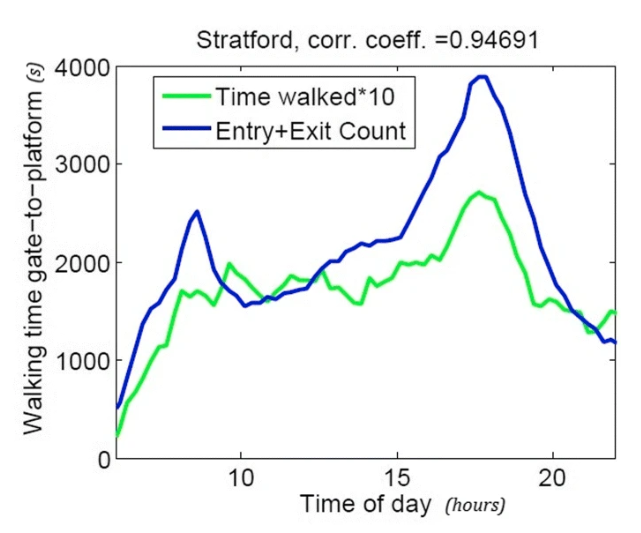
\includegraphics[width=0.5\textwidth]{London_Walking_time.png}%
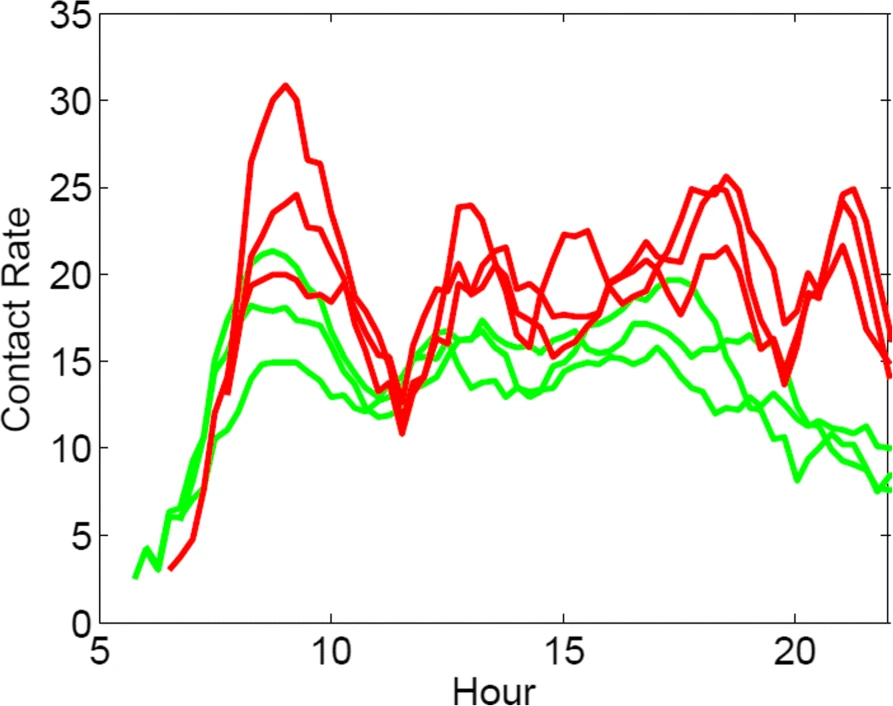
\includegraphics[width=0.5\textwidth]{London_Borough_Comparison.png}
\textit{Results show a correlation between the use of the underground and ILI cases in London, specifically they show that higher numbers of ILI cases arise in those boroughs where the population spend more time in the Underground and/or incur in a higher number of contacts when travelling.}
 \cite{gosce_johansson_2018}
\end{frame}
\begin{frame}
\frametitle{COVID in London}
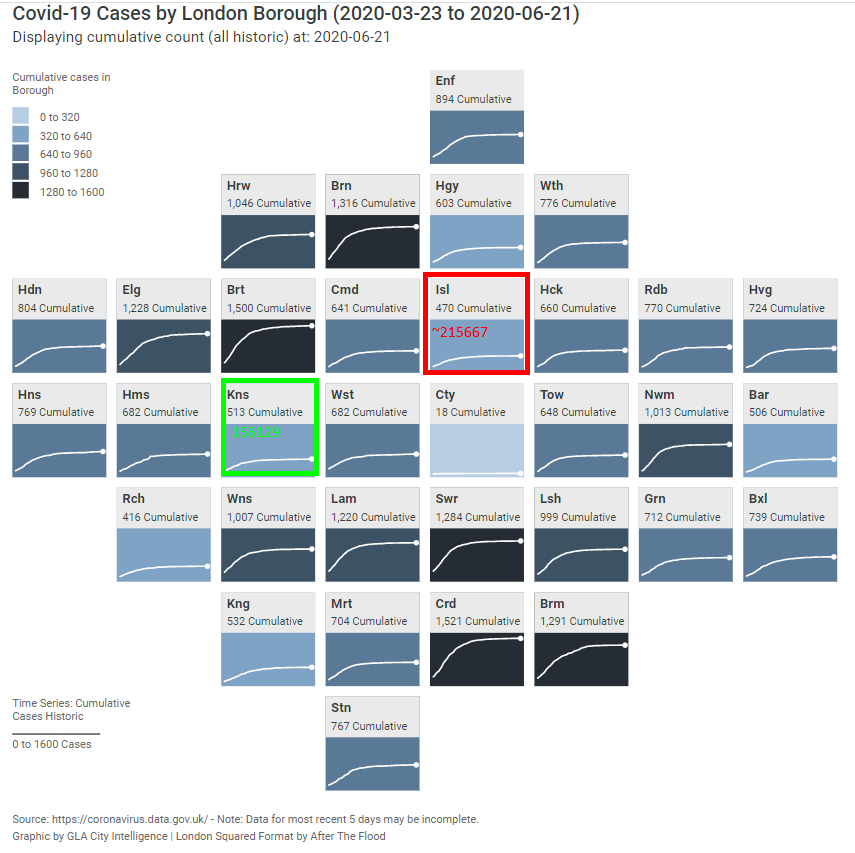
\includegraphics[width=0.7\textwidth]{London_Covid_Adapted.png}
\textit{Speaker's Remark: Boroughs of NY != Boroughs of London}
\end{frame}
\begin{frame}
\frametitle{Prior Research (Singapore Buses)}
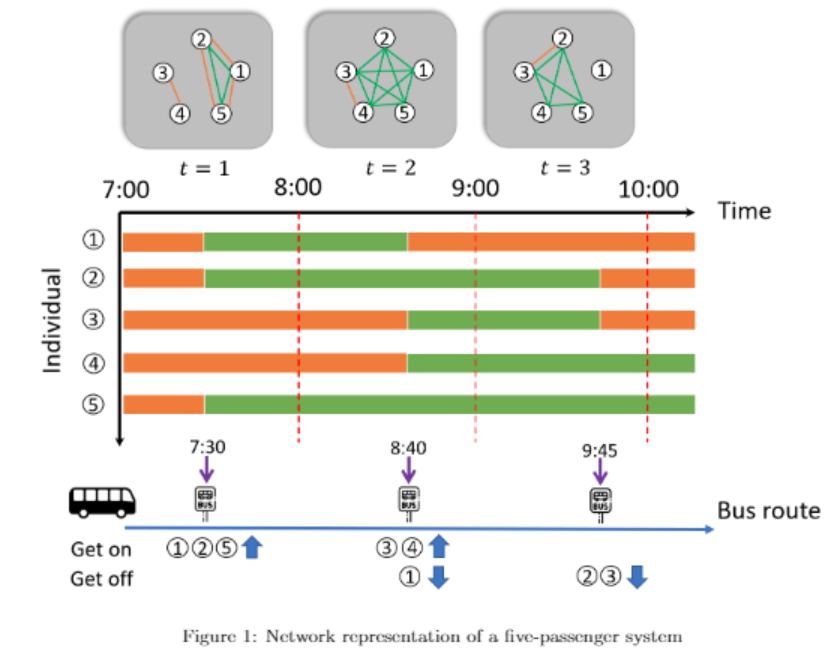
\includegraphics[width=0.5\textwidth]{Singapore_1.png}%
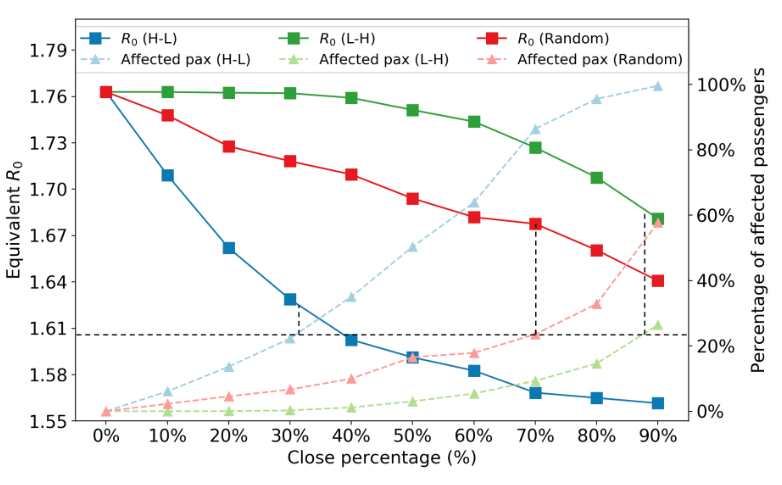
\includegraphics[width=0.5\textwidth]{Singapore_2.png}
\textit{The direct contact in trains is, however, difficult to obtain from smart card data because the transactions are recorded at the station level}
\cite{singapore_bus_2020}
\textit{Speaker's note:\\
- We show these things not to embarrass ourselves, but the depth of research available even just looking at one system.
- List some other research
}
\end{frame}
\begin{frame}
\frametitle{ABM Framework}
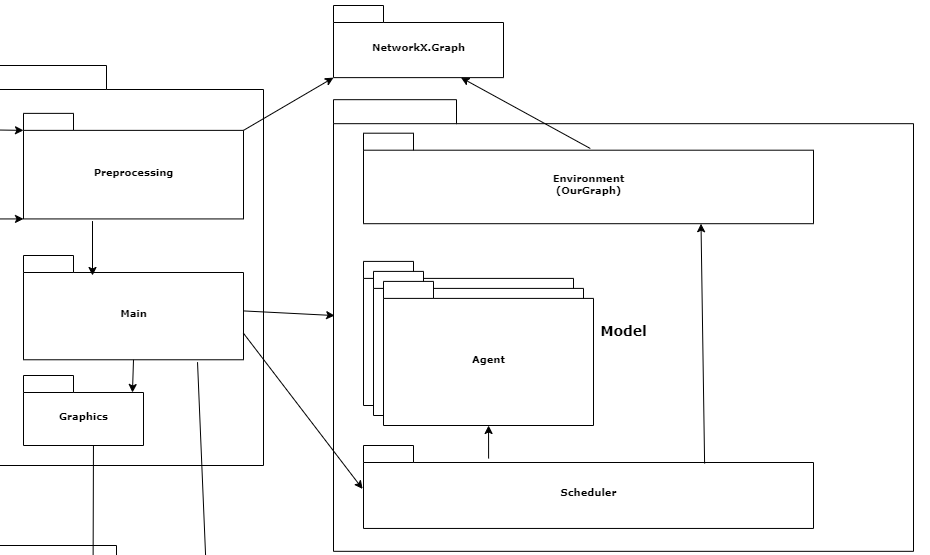
\includegraphics[width=1.0\textwidth]{covid_framework_summary.png}
Components: Python, MESA, Networkx

Transportation Model\\
SEIR Agent\\
\textit{Speaker's Notes:\\
Me no good math. me simulate.
much result wow.}
\end{frame}
\begin{frame}{Embedded Animation}
\frametitle{Simple Geometries}
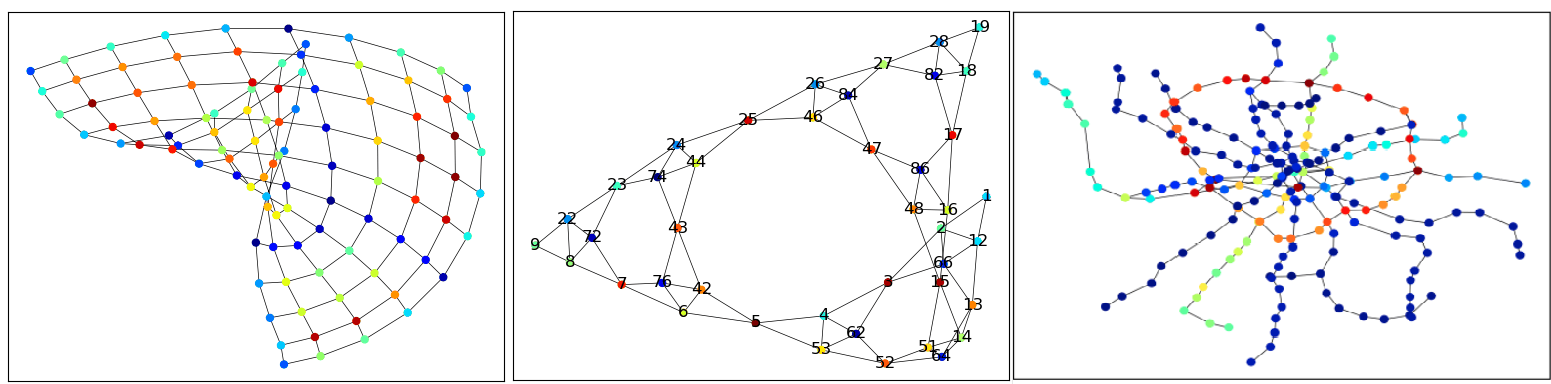
\includegraphics[width=1.0\textwidth]{geometries_example.png}
\begin{itemize}
    \item \href{https://github.com/cheung-ho-lum/NS_Epidemics_ABM_Approach/blob/master/Repository/Visualizations/infection_timelapse_grid_01.gif}{Grid}
    \item \href{https://github.com/cheung-ho-lum/NS_Epidemics_ABM_Approach/blob/master/Repository/Visualizations/infection_timelapse_sierpinski_01.gif}{Sierpinski's Triangle}
    \item \href{https://github.com/cheung-ho-lum/NS_Epidemics_ABM_Approach/blob/master/Repository/Visualizations/infection_timelapse_moscow.gif}{Moscow}
\end{itemize}
\end{frame}
\begin{frame}
\frametitle{World Airline Network (Passenger Flow)}
Data Source (openflights, articles)
Methods (ABM)
\end{frame}
\begin{frame}
\frametitle{World Airline Network (Passenger Flow)}
\end{frame}
\begin{frame}
\frametitle{Madrid Commuter Trains (Central Hubs)}
Data Source (madrid renfe gtfs)
Methods (ABM)
\end{frame}
\begin{frame}
\frametitle{Results (Madrid)}
\end{frame}
\begin{frame}
\frametitle{NYC COVID Demographics}
\end{frame}
\begin{frame}
\frametitle{Subway Systems}
\end{frame}
\begin{frame}
\frametitle{NYC Subway Data}
\textit{90\% loss.}
\end{frame}
\begin{frame}
\frametitle{NYC Subway Modeling}
\end{frame}
\begin{frame}
\frametitle{NYC Model Hyper-parameters}
\end{frame}
\begin{frame}
\frametitle{Compartmental Modeling Results (NYC)}
\end{frame}
\begin{frame}
\frametitle{Results by MODZCTA (NYC)}
\end{frame}
\begin{frame}
\frametitle{Discussion}
All models are wrong!\\
- Passenger Flow
- Outer suburbs phenomenon exists
- Simple GDP/capita data
\end{frame}
\begin{frame}
\frametitle{Conclusions}
\end{frame}
\begin{frame}
\frametitle{Credits, Links, References}
Frank Acquaye - WAN, Passenger Flow\\
Ho Lum Cheung - NYC, Organization, Research, Testing\\
Dimas Muñoz-Montesinos - Madrid, Hotspots\\
Elie Wanko - Theory, Consulting\\
github link
references used in slides
\bibliography{bib_file}{}
\bibliographystyle{plain}
\end{frame}
\end{document}
